\section{Introduction}
\label{sec::introduction}


\begin{figure*}[htbp]
    \centering
    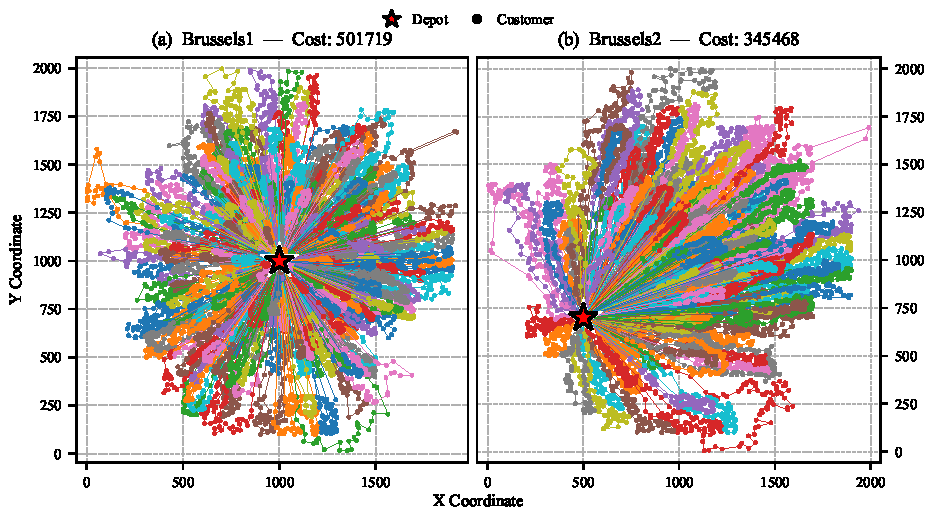
\includegraphics[width=\textwidth, height=0.4\textheight]{assets/BKS_Brussels1_Brussels2_combined.pdf}
    \caption{Best Known Solution (BKS) for Brussels instances from CVRPLIB~\cite{CVRPLIB}, exhibiting a flower-like routing pattern}
    \label{fig:BKS_Brussels}
\end{figure*}

%The Capacitated Vehicle Routing Problem (CVRP) is a fundamental combinatorial optimization problem in which a fleet of vehicles with limited capacity must serve a set of customers with known demands, starting and ending at a central depot, while minimizing the total routing cost.

The Capacitated Vehicle Routing Problem (CVRP) is a fundamental combinatorial optimization problem. 
It involves a fleet of vehicles with limited capacity that serve a set of customers with known demands, starting and ending at a central depot, while minimizing the total distance traveled. Algorithms developed for CVRP are widely applicable to transportation and delivery optimization problems. Several variants of CVRP have been studied, including environmentally aware formulations that minimize carbon emissions \cite{Bektas_Laporte_PRP} and variants with customer time window constraints \cite{Solomon_VRPTW}. The NP-hard nature of the problem renders exact approaches impractical for large instances, motivating the use of approximation algorithms and heuristic methods. Due to the practical importance and theoretical challenge posed by CVRP, it has received significant attention in the literature~\cite{pecin2017new, arnold2019efficiently}. Unfortunately, most of these studies are limited to relatively smaller instances. The approximation algorithms and heuristics primarily target instances with only a few hundred to a few thousand customers. In the logistics sector, while small and medium instance sizes permit optimizing for local warehouses, optimizing across multiple cities and countries necessitates a global consideration involving millions of customers. However, theoretical bounds and practical limitations prevent the existing efficient methods from scaling.

Our goal in this work is to design a solver for million-scale CVRP. In particular, we propose finding a solution to large CVRP instances within minutes without adversely affecting the solution quality. Our method utilizes a new parallel divide-and-conquer algorithm to decompose the geometry into smaller instances, to solve them concurrently via a minimum spanning tree construction, and to escape the local extrema via randomization. The main contributions of this paper are as follows.

1) \textbf{Parallel Divide-and-Conquer Framework with Strong Scalability}: 
We propose a spatial decomposition-based approach that first partitions the problem into independent subproblems, followed by MST-guided route construction within each partition and randomized DFS-based exploration. The method exhibits strong scalability with respect to both problem size (up to million-scale instances) and parallel execution on multi-core architectures.

2) \textbf{Open-Source Parallel Implementation}\footnote{Publicly available source code: \url{https://github.com/CodeCraftsmanSandeep/BP-MDS}}: We provide an optimized OpenMP-based parallel CPU implementation, called BP-MDS, which incorporates efficient load balancing, on-demand memory allocation, and a customized min-heap design that avoids constructing the complete graph, resulting in significant reductions in CVRP execution time and memory consumption.

3) \textbf{Thorough Experimental Evaluation}: 
We demonstrate that our algorithm efficiently solves million-scale CVRP instances, handling inputs of up to 5 million nodes within 8 minutes. Across standard benchmark datasets, BP-MDS achieves an overall geometric mean optimality gap of 8.51\% 
(9.67\% on CVRPLIB~\cite{CVRPLIB} (130 instances) and 1.27\% on FILO2~\cite{FILO2} (20 instances)).

